\subsection{Исследование неподвижных точек на устойчивость}

Для начала определим все нужные нам понятия. Пусть задана система
\begin{equation} \label{CommonOneStepSystem}
        u_{t+1} = f(u_t), \; где \; f:\R\rightarrow\R,\; t = 0,\: 1,\: 2,\: \dots 
\end{equation}

\begin{definition}
        Множество точек $u_t,\; t = 0,\: 1,\: 2,\: \dots$ называется траекторией (или~орбитой) системы, порожденной отображением~$f$. \cite[стр.~82]{bratus10}
\end{definition}

\begin{definition}
        Неподвижная точка~$u^*$ системы \ref{CommonOneStepSystem} называется устойчивой по~Ляпунову, если для~любого $\varepsilon > 0$, существует такое $\delta=\delta(\varepsilon) > 0$, что~для~любых начальных данных $u_0$ из~$\delta$-окрестности точки $u^*$ вся траектория системы $u_t,\; t = 0,\: 1,\: 2,\: \dots$ содержится в~$\varepsilon$-окрестности точки $u^*$. Если, кроме~того, $\lim\limits_{t \to \infty} f(u_t) = u^*$, то~точка~$u^*$ называется асимптотически устойчивой. \cite[стр.~82]{bratus10}
\end{definition}
            
\textit{Замечание.} Ассимптотически устойчивые неподвижные точки иногда называют \textit{аттракторами}, а~неустойчивые неподвижные точки~--- \textit{репеллерами}. \cite[стр.~83]{bratus10}
            
\begin{theorem} \label{th:stability}
        Задана система~\ref{CommonOneStepSystem}. Пусть $f$~--- непрерывно дифференцируемая функция, $u^*$~--- неподсижная точка системы~\ref{CommonOneStepSystem}. Тогда
        \begin{enumerate}
                \item если $|f'_u(u^*)| < 1$, то $u^*$ асимптотически устойчива;
                \item если $|f'_u(u^*)| > 1$, то $u^*$ неустойчива;
                \item если же $|f'_u(u^*)| = 1$, то про~устойчивость точки~$u^*$ ничего сказать нельзя.
        \end{enumerate}
        \cite[стр.~83]{bratus10}
\end{theorem}

Итак, перейдем к~исследованию на~устойчивость неподвижных точек системы~\ref{eq:first_discrete_system}. Напомним, что~она имеет следующий вид
$$
        u_{t+1} = r u_t^2 e^{-u_t},\; u_t > 0,\; \forall t = 0,\; 1,\: 2,\: \dots .
$$
Для~данной системы функция $f(u) = r u^2 e^{-u}$ непрерывно дифференцируемая на всей области определения ($u \geqslant 0 $) системы \ref{eq:first_discrete_system}, следовательно, можно применить теорему \ref{th:stability}. Найдем производную функции $f$.
\begin{equation} \label{OneStepDeriv}
        f'_u(u) = r (2u e^{-u} - u^2 e^{-u}) = r u e^{-u} (2 - u)
\end{equation} 

Видно, что для $u^* = 0$, неподвижной точки, существующей при всех значения параметра, $|f'_u(u^*)| = 0$ для~любого $r > 0$. Значит, $u^*$ является аттрактором.

Исследуем на устойчивость остальные неподвижные точки. Напомним, что они являются решением уравнения \ref{eq:fix_point_equation}
$$
        u^* e^{-u^*} = \frac{1}{r}.
$$
Поэтому мы можем преобразовать производную \ref{OneStepDeriv}
\begin{equation}
        f'_u(u^*) = r \frac{1}{r} (2 - u^*) = 2 - u^*.
\end{equation}

Получается, что
\begin{enumerate}
        \item $|f'_u(u^*)| > 1$ при $u^* \in (1, 3)$;
        \item $|f'_u(u^*)| < 1$ при $u^* \in (0, 1) \cup (3, +\infty)$;
        \item $|f'_u(u^*)| = 1$ при $u^* \in \{1, 3\}$.
\end{enumerate}
            
При $r = e$ есть только одна неподвижная точка $u^* = 1$, и сделать вывод о ее устойчивости методами линейного анализа не представляется возможным. При $r > e$, появляются две неподвижные точки $0 < u_1^* < 1$ и $u_2^* > 1$. $u_1^*$ всегда неустойчива, при этом $u_2^*$ неустойчива при $e<r<\frac{e^3}{3}$, асимптотически устойчива при $r > \frac{e^3}{3}$. При $r = \frac{e^3}{3}$ об устойчивости точки $u_2^*$ ничего сказать нельзя. Посмотреть на это можно на нижеприведенных графиках.

\begin{figure}[h!]
        \centering
        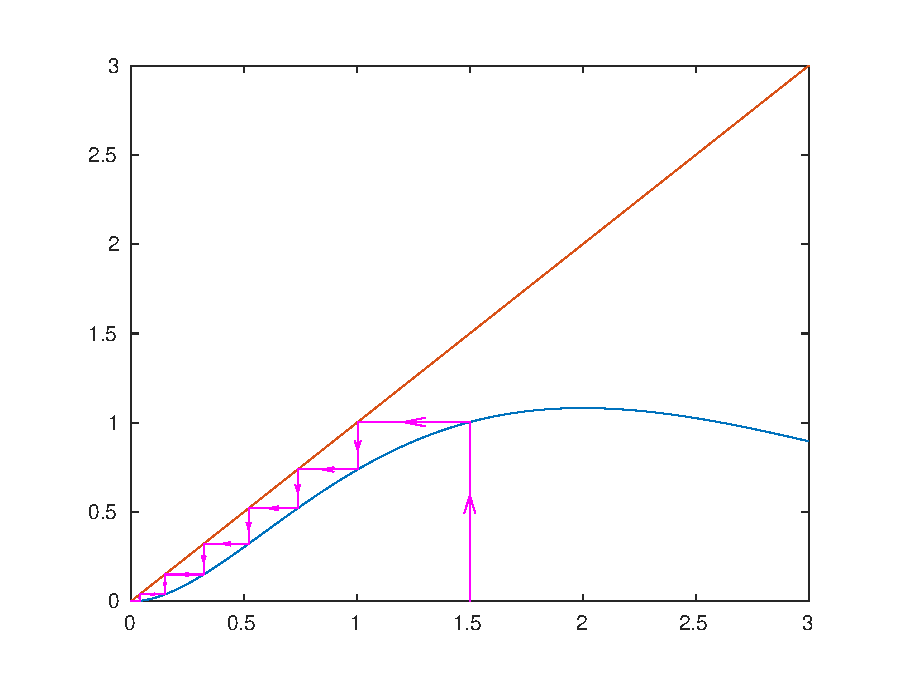
\includegraphics[width=0.8\linewidth]{first_discrete_system/stability_of_fixed_points/r2start1-5.eps}
        \caption{Орбита системы \ref{eq:first_discrete_system} при $r = 2$, $u_0 = 1,5$.}
\end{figure}
\begin{figure}[h!]
        \centering
        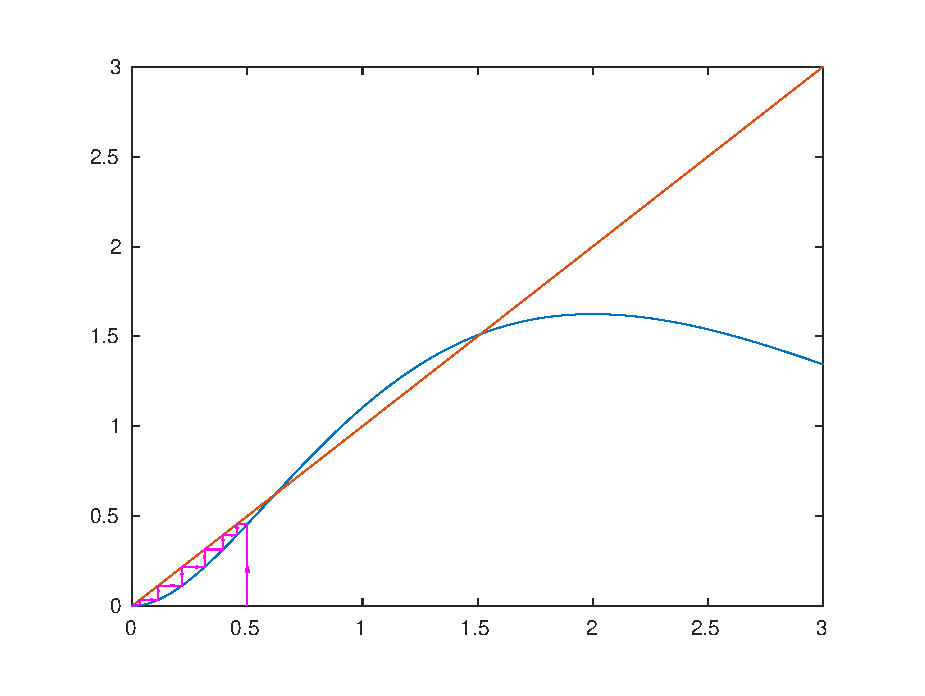
\includegraphics[width=0.8\linewidth]{first_discrete_system/stability_of_fixed_points/r3start0-5.eps}
        \caption{Орбита системы \ref{eq:first_discrete_system} при $r = 3$, $u_0 = 0,5$.}
\end{figure}
\begin{figure}[h!]
        \centering
        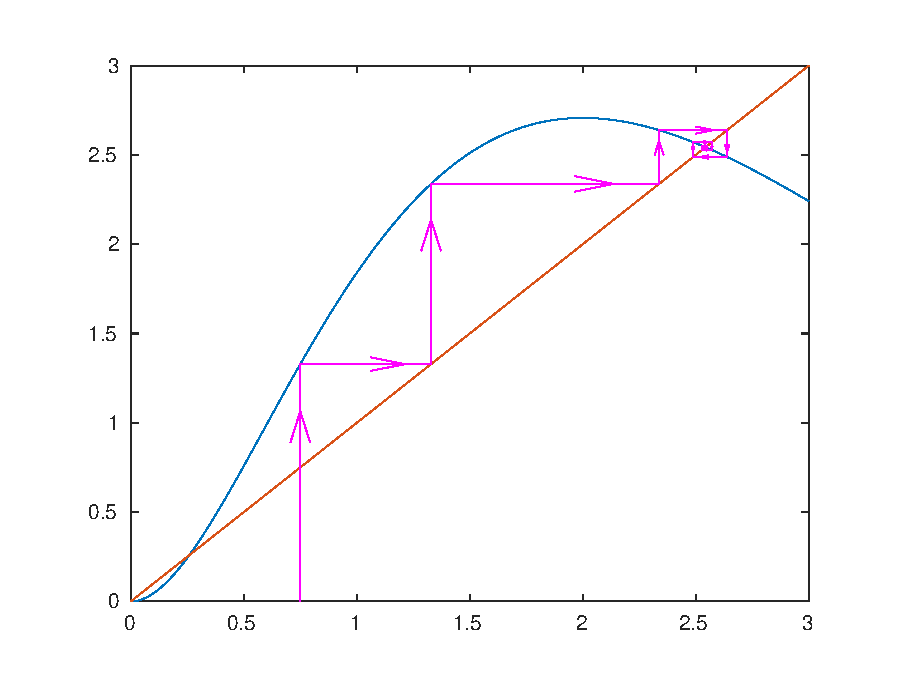
\includegraphics[width=0.8\linewidth]{first_discrete_system/stability_of_fixed_points/r5start0-75.eps}
        \caption{Орбита системы \ref{eq:first_discrete_system} при $r = 5$, $u_0 = 0,75$.}
\end{figure}
\begin{figure}[h!]
        \centering
        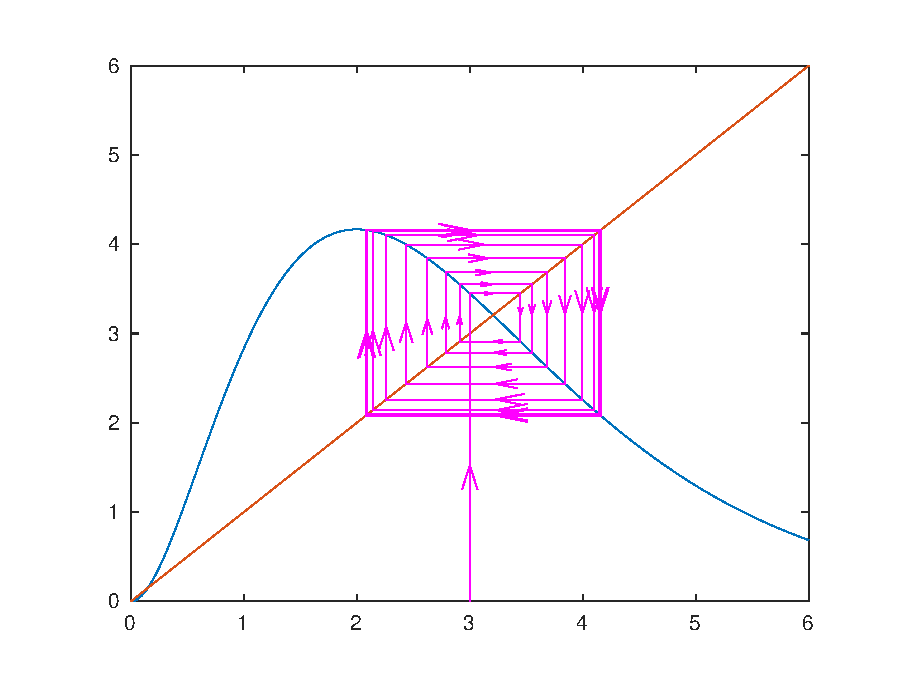
\includegraphics[width=0.8\linewidth]{first_discrete_system/stability_of_fixed_points/re3div3plus1start3.eps}
        \caption{Орбита системы \ref{eq:first_discrete_system} при $r = \frac{e^3}{3} + 1$, $u_0 = 3$.}
\end{figure}
\clearpage